\chapter{Monte Carlo Search}
\label{chap:monte}
\section{Introduction to Monte Carlo experiments}
Monte Carlo experiments are a class of 
computational algorithms that rely on repeated random sampling to compute 
their results. Monte Carlo methods are often used in computer simulations 
of physical and mathematical systems. These methods are most suited to 
calculation by a computer and tend to be used when it is infeasible to 
compute an exact result with a deterministic algorithm. This method is 
also used to complement theoretical derivations. 
In an Monte Carlo search, input values are drawn from some probability 
distribution, say the normal or the Poisson distributions. The 
corresponding output values are computed and compared. The distribution 
used may affect the quality of the results, and should be chosen 
carefully. 

\section{Random Searches vs. Sequential Searches}
Using a fixed grid for searching the space of stable filters has its 
pitfalls. For one, as can be seen from the figures of the previous 
chapter, as one moves further away from the origin in the \gls{cpc} plane, 
the lines move further apart. It is not easy to provide a gradient to the 
intervals in which the range of \gls{t} is discretized, since different 
systems have different spaces of stable filters. So far, in the cases 
studied, the area of stable filters seems to be dense around the origin, 
both for 2D and 3D systems. But it is difficult to predict which values of 
\gls{t} correspond to \glspl{cpc} near the origin. Sometimes, values of 
\gls{t} corresponding to the points in the stable region might lie quite 
far from the origin, in which case sequential search would go a long while 
without yielding stable points, whereas an uniform distribution Monte 
Carlo search could chance upon stable points much sooner, as it looks at 
the entire grid.

Using the 2D system presented in \autoref{sec:2d}, a comparison of the number 
of stable points discovered by both sequential and Monte Carlo (uniform 
distribution) searches was made. The result can be seen in \autoref{fig:c2d}. 
The Monte Carlo method provided a constant stream of stable points, where 
as the sequential search had bursts of rapid success followed by plateaus 
of stagnation. Indeed, the sequential search showed no increase in the 
number of stable points for around 500,000 points during each period of 
stagnation. Also, a number of stable points were discovered by the Monte 
Carlo search in the gaps left by the sequential search (while, of course, 
missing points found by the sequential search).

We theorize that the apparent gaps in the region of stable filters, apart 
from the unreachable region discussed in \autoref{sec:un}, is due to the 
fixed, uniform discretization used in the sequential search, and the gaps 
apparent in  \cite[Fig. 4-10]{Jiffri2011} would not have followed the 
distinctive pattern, had a Monte Carlo search been used. Indeed, a glance 
at \autoref{fig:comp} will reveal that some pattern is apparent in the 
sequential search results, whereas nothing of the sort is visible in the 
results of the Monte Carlo experiment.
\begin{figure}
\subfloat[Monte Carlo method]{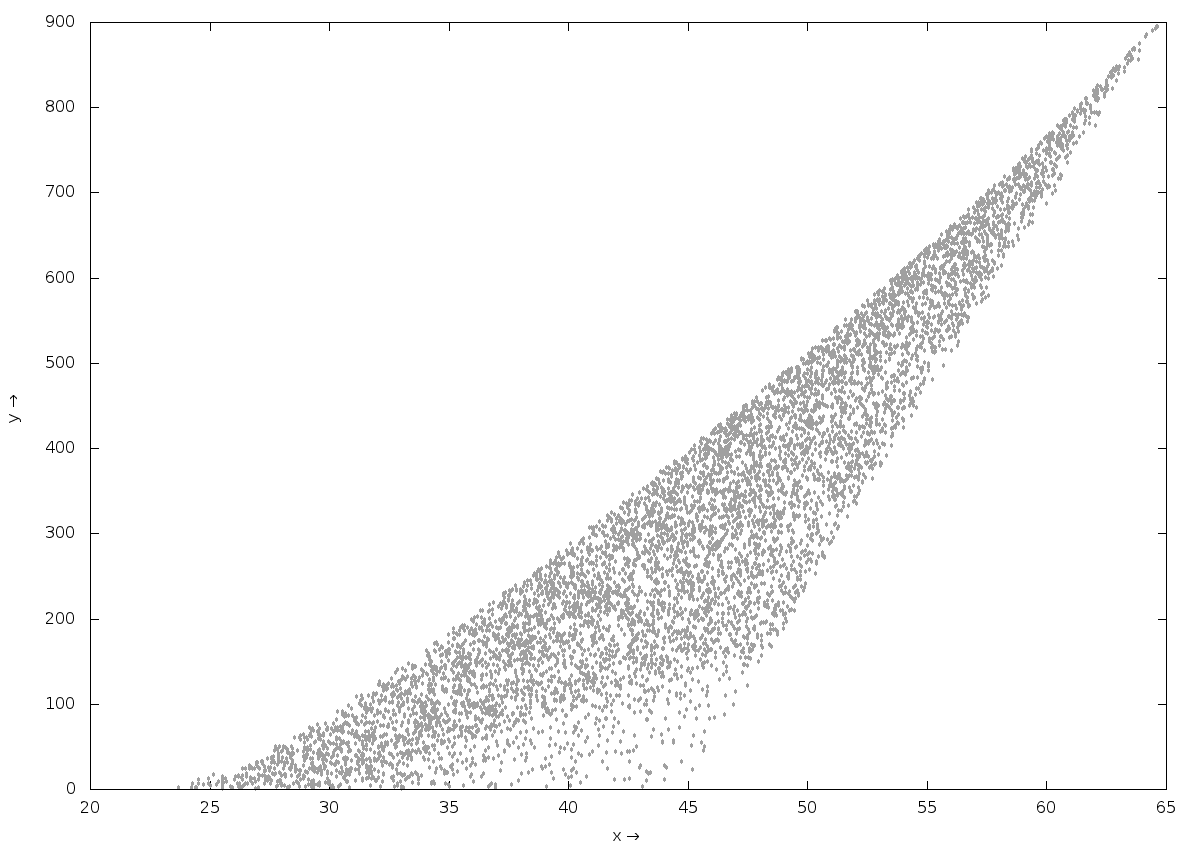
\includegraphics[width=0.48\textwidth]{ran.png}}
\subfloat[Sequential search]{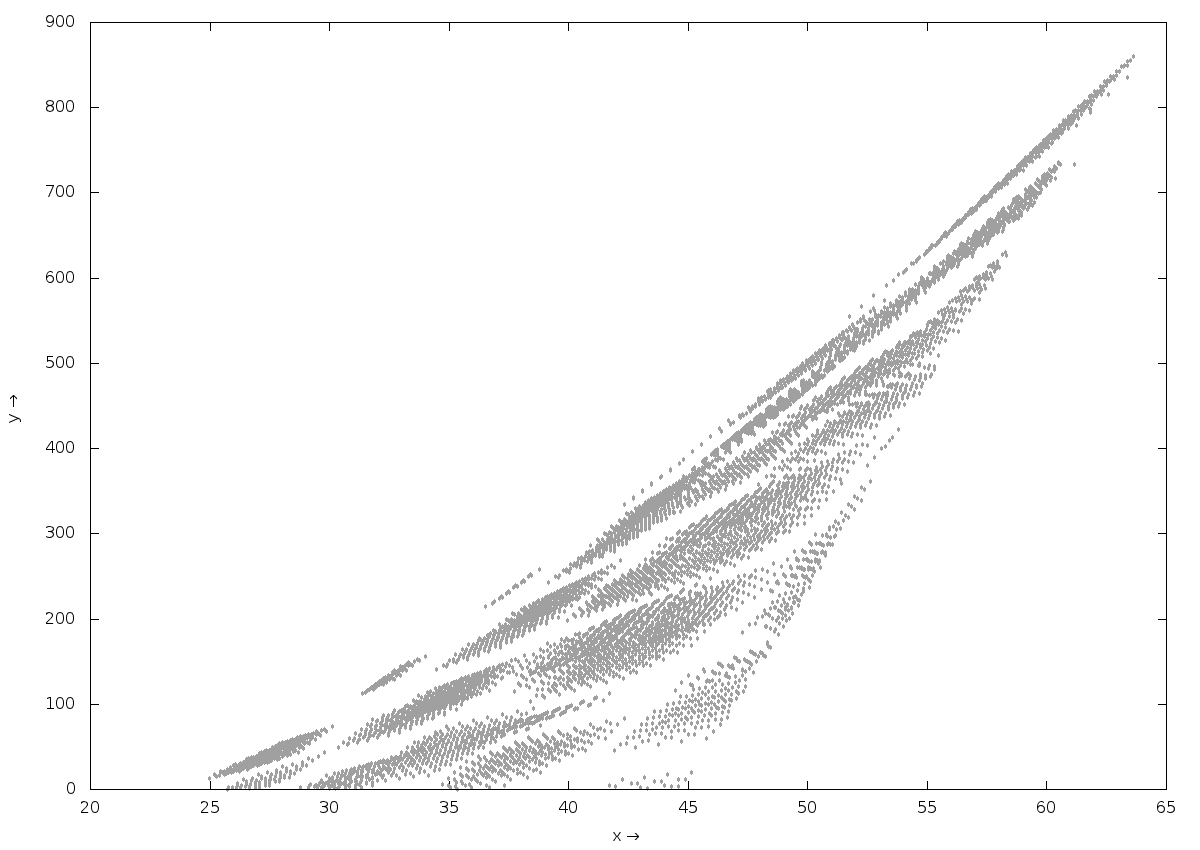
\includegraphics[width=0.48\textwidth]{seq.png}}
\caption{Comparison of Stable Points returned by Monte Carlo and Sequential searches}
\label{fig:comp}
\end{figure}
Interestingly, a comparison of Monte Carlo searches using different 
distributions does not show such differences. Both uniform and normal 
distribution show similar performance, the normal distribution being just 
slower than the uniform distribution for the same 2D system. However, the 
regions of \gls{t} evaluated by each prove insightful. In both cases, (see 
\autoref{fig:theta}), the points corresponding to stable \glspl{cpc} are 
clustered in rectangular regions around some points which are located over 
a repeating pattern. So a possible way to speed up the search for stable 
points would be to do a Monte Carlo search using the uniform distribution 
to obtain a small number of initial, evenly spread points, and then 
execute searches using the normal distribution centred over these seed 
points.
\begin{figure}
\centering
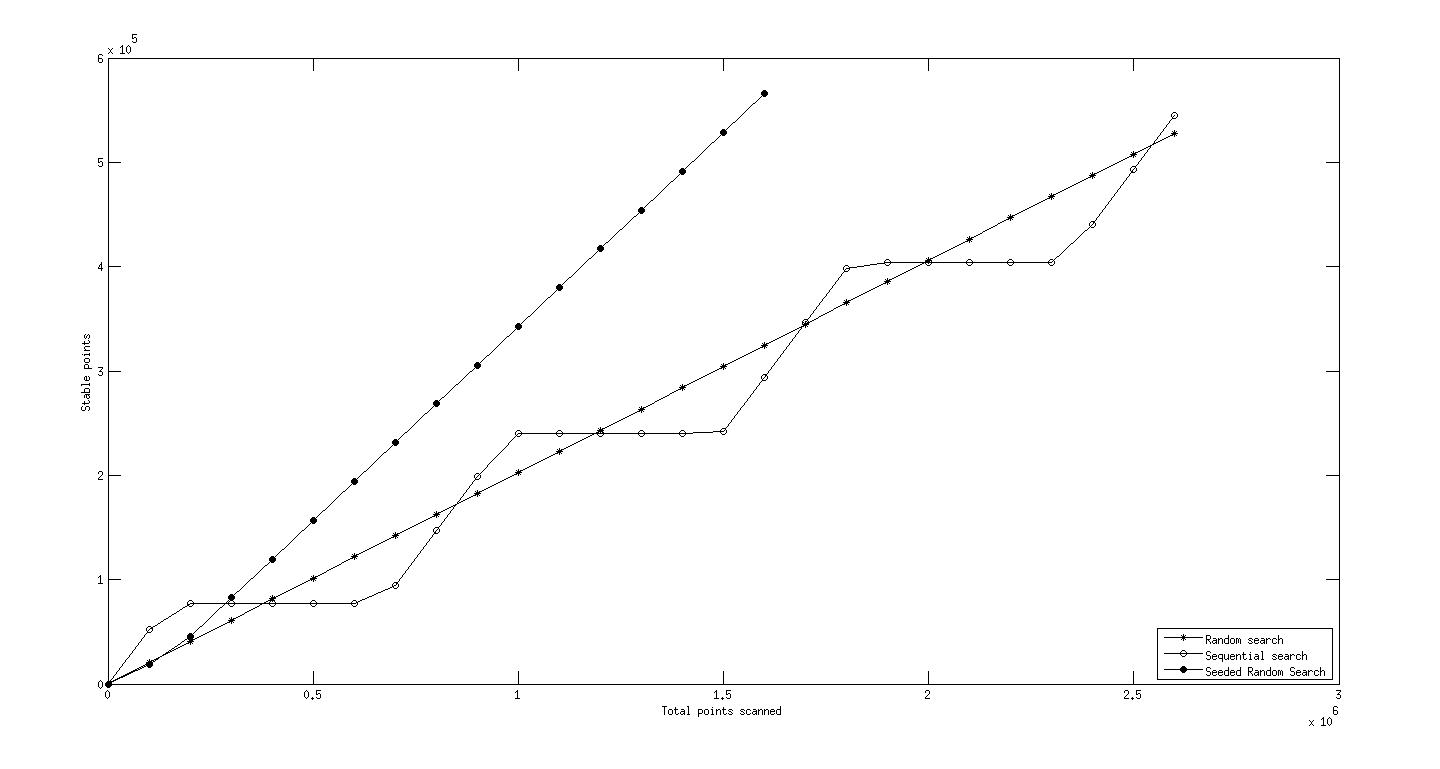
\includegraphics[width=\textwidth]{seed.jpg}
\caption{Number of stable points discovered vs total number of points examined}
\label{fig:c2d}
\end{figure}

In fact, this does considerably speed up the search process. Depending 
upon how many seed points were generated, the process would accelerate 
sharply after a certain stage, and produce around 36,000 stable points for 
every 100,000 points discarded, whereas just using one distribution would 
only produce around 18,000 stable points per 100,000 discarded -- a speed-up
by a factor of 2. The stage at which this sudden increase in rate of 
discovery occurs can be pushed back to happen earlier by using fewer seed 
points. The optimum number of seed points seems to be around 10,000, with 
both 5000 and 20,000 points showing the speed-up at a later stage. A 
comparison of the rates of this Monte Carlo method (with 5,000 
seed points) with the uniform distribution and the sequential search of 
is presented in \autoref{fig:c2d} .

Though the Poisson distribution has not been used so far, it has its 
applications. Given a grid over the region of \gls{t}, one can use the 
Poisson distribution to select random grid points for evaluation. This may 
increase the rate of discovery of stable points. Also, one may combine the 
Poisson distribution with seed points from uniform distribution like we 
have done for the normal, and perhaps obtain a better method than even the 
previous one.